\chapter[Wägeeinrichtung (Viertelbrücke)]{Aufbau einer Wägeeinrichtung mit dem Biegestab (Viertelbrücke)}

Eine Wägeeinrichtung mit Brückenschaltung ist nach Schaltskizze \ref{cir:quarter-bridge}
aufzubauen und zu untersuchen.
Für \( R_1 \) ist der Widerstand \( R_1 \) der 4 Dehnungsmessstreifen-Widerstände
des Biegebalkens zu verwenden.
\( R_3 \) und \( R_4 \) sind Präzisionswiderstände mit
\begin{align}
    R_3 = R_4 = 1 \si{\kilo\ohm} \quad (0.02 \% \quad \text{Toleranz})
\end{align}
aus dem \textit{hps Board}.
Die Versorgunsspannung beträgt \( U_0 = 6 \si{\volt} \).
Die Brückenspannung \( U_{ab} \) wird mit einem Digitalmultimeter \textit{METRAHit TECH} gemessen.

\begin{figure}[!h]\centering
    \vspace*{0.7cm}
    \begin{circuitikz}[american, scale = 0.7]
    \draw
    (0,0) to[european voltage source, l=$U_0$] (0,6)

    (0,6) to[short, -*] (6,6)
          to[variable resistor, l=$R_1$] (6,3)

    (6,6) to[short, -] (12,6)
          to[resistor, l=$R_3$] (12,3)

    (6,3) to[short, *-o] (7,3)
    (7,3) node[label=$a$] {}
    (12,3) to[short, *-o] (11,3)
    (11,3) node[label=$b$] {}

    (7,3) to[voltmeter, l=$U_{ab}$] (11,3)

    (6,3) to[resistor, l=$R_2$] (6,0)
    (12,3) to[resistor, l=$R_4$] (12,0)

    (0,0) to[short, -*] (6,0)
          to[short, -] (12,0)

    % (2.5,6.2) node[label={[font=\footnotesize]east:$I_M$}] {}
    % (4.3,4) node[label={[font=\footnotesize]east:$U_M$}] {}

    % (7.5,4) node[label={[font=\footnotesize]east:Long distance}] {}
    ;
    \end{circuitikz}
    \caption{Wägeeinrichtung (Viertelbrücke)} \label{cir:quarter-bridge}
\end{figure}

Die Brückenspannung ist ohne Belastung des Biegebalkens
durch Variation von \( R_2 \) so gut wie möglich
auf \( U_{ab} = 0 \si{\volt} \) abzugleichen.
Es ist die Brückenspannung \( U_{ab} \) bei Belastung des Biegebalkens mit:
\begin{align}
    m = 0 \si{\gram}, 100 \si{\gram}, 200 \si{\gram}, 300 \si{\gram}, 400 \si{\gram}, 500 \si{\gram}
\end{align}
zu messen.
Die Empfindlichkeit der Anordung für \( m = 500 \si{\gram} \) ist zu bestimmen.

\section[Vorbereitung]{Vorbereitung}
Siehe Berechnungsgrundlagen für Brückenempfindlichkeit.

\section[Messung]{Messung}
Die Schaltung wurde gemäß der Versuchsbeschreibung aufgebaut.
Der Biegebalken ist unbelastet.
Die Widerstandsdekade \( R_2 \) wurde stufenweise verstellt,
bis das Multimeter einen Abgleich von \( 0 \si{\volt} \) anzeigt hat.

Der Biegebalken wurde nacheinander mit den Gewichten
\( m = 0 \si{\gram}, 100 \si{\gram}, 200 \si{\gram}, 300 \si{\gram}, 400 \si{\gram}, 500 \si{\gram} \)
belastet und die Brückenspannung \( U_{ab} \) wurde vom Multimeter abgetragen.
Die Empfindlichkeit der Brücke wurde für \( m = 500 \si{\gram} \) errechnet.

\section[Messdaten]{Messdaten}

\begin{align*}
    R_1 \quad \text{at} \quad 0 \si{\ohm} &= 700.7 \si{\ohm} \\
    R_2 &= 700.3 \si{\ohm}
\end{align*}

\begin{table}[!h]
    \centering
    \begin{tabular}{rrr}
    \toprule
        ~                 & \multicolumn{1}{c}{METRAHit TECH}    \\
        ~                 & \multicolumn{1}{c}{(U) Voltage}      \\
    \midrule
          0\si{\gram}      &  0.0000\si{\volt}  \\
        100\si{\gram}      & -0.0004\si{\volt}  \\
        200\si{\gram}      & -0.0006\si{\volt}  \\
        300\si{\gram}      & -0.0008\si{\volt}  \\
        400\si{\gram}      & -0.0011\si{\volt} \\
        500\si{\gram}      & -0.0013\si{\volt} \\
        ~ & ~ \\
    \bottomrule
    \end{tabular}
    \caption{Spannungsmessung der Viertelbrücke.}
    \label{tab:quarter-bridge-voltage-measurement}
\end{table}

\begin{figure}[!h]
    \centering
    \begin{tikzpicture}
        \begin{axis}
            [
                xlabel={[g] Weight},
                ylabel={[V] Voltage},
                grid,
                xmin=0,
                xmax=500,
                ymin=-0.002,
                ymax=0.002,
                samples = 50,
                domain=0:500,
                legend pos=north east,
                tick align=inside
            ]
            \addplot[cyan, mark=asterisk, smooth, ultra thick] table[col sep=comma, x=weight, y=voltage]{./data/measurement_quarter_bridge.csv};

            \addlegendentry{($U_{ab}$) Messung}

        \end{axis}
    \end{tikzpicture}
    \caption{Plot der Spannungsmessung der Viertelbrücke.}
    \label{fig:quarter-bridge-voltage-measurement}
\end{figure}

\section[Auswertung]{Auswertung}

Die systematische Erhöhung der Belastung führt zu einem steigenden Widerstand \( R_1 \),
weshalb sich auch die Brückenspannung \( U_{ab} \) erhöht.
Die Brückenempfindlichkeit ist mit
\begin{align}
    E_0 &= 0.00214 \si{\volt\per\ohm}
\end{align}
eher gering, da der Widerstand \( R_1 \) relativ hoch ist
und die Eingangsspannung \( U = 6 \si{\volt} \) gering ist.
Die Brückenempfindlichkeit ist somit unabhängig von dem eingesetzten Gewicht
und der dadurch resultierenden Widerstandeserhöhung.
\subsection[Simulation]{Simulation}
In einer zusätzlichen Simulation mit falstad.com
- unter Optimal-Bedingungen ohne Messfehler und Widerstandstoleranzen -
wurden die Messergebnisse näherungsweise überprüft.
Der Widerstandswert für \( R_1 \) bei \( 500 \si{\gram} \) wurde 
approximiert, da kein direkter Messwert vor lag.

Da:
\begin{alignat*}{3}
    & R_1 \quad &&\text{bei} \quad 0g   &&= 700.7 \si{\ohm} \\
    & R_1 \quad &&\text{bei} \quad 200g &&= 700.8 \si{\ohm}
\end{alignat*}
wird bei ansatzweiser linearer interpolation
\begin{alignat*}{3}
    & R_1 \quad &&\text{bei} \quad 500g &&\approx 701 \si{\ohm}
\end{alignat*}
liegen.

\begin{figure}[!h]
    \centering
    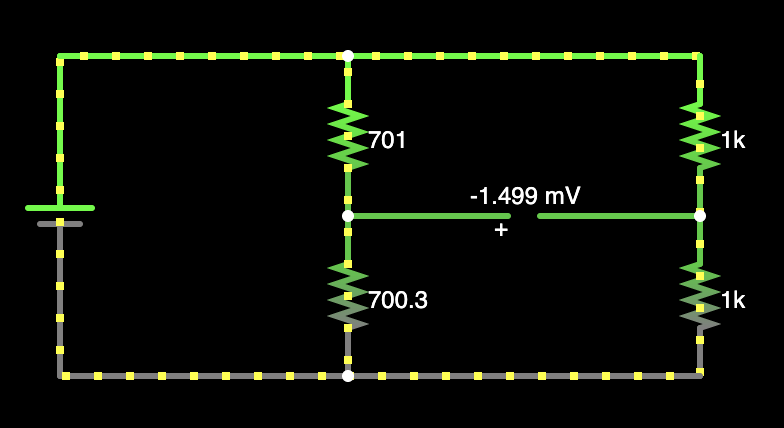
\includegraphics[width=0.6\textwidth]{./figs/04_falstad_black.png}
    \caption{Simulation der Viertelbrücke.}
    \label{fig:quarter-bridge-simulation}
\end{figure}

Die Brückenspannung \( U_{ab} \) beträgt \( -1.449 \si{\milli\volt} \approx -0.0014 \si{\volt} \).
